\newpage
\section{Differenzierer}
Zuerst wurde die folgende Schaltung realisiert:
\begin{figure}[h]
    \centering\begin{circuitikz}[european resistors]
        \draw(0,0) node[op amp, yscale=-1] (opamp){};
        \draw (opamp.+) to [C=$C_1$,-o,i_<=$I_1$] ++(-3,0) to [open,v>=$U_\text{e}$] ++(0,-3) to [short,o-] ++(2,0) to node[ground](gnd){} ++(0,0);
        \draw (opamp.-) to [short] ++(-1,0) to [short] ++(0,-1) to node[short](r2){} ++(0,0) to [short,-*] (gnd);
        \draw (gnd) to [short,-o]++(5.35,0) to node[short,-o](end){}++(0,0);
        \draw (opamp.out) to node[short,*-*](r1){} ++(1,0) to [short,-o] ++(1,0) to [open,v>=$U_\text{a}$] (end);
        %\draw (r1) to [short,*-,i>^=$I_2$]++(0,-1.5) to [R=$R_2$,v>=$U_2$] (r2);
        %\draw (r2)++(0,1) to [open] ++(-1,0) to node[short](o1){} ++(0,0)to[open,v>=$U_1$]++(0,-3);
        %\draw (o1) to [open,v^<=$U_3$]++(0,1);
        \draw (opamp.out) to [short,*-]++(0,2) to [R=$R_2$,i>=$I_2$]++(-2.35,0) to [short,-*] (opamp.+);
    \end{circuitikz}
    \caption{Schaltplan der einfachen Differenzierschaltung}
\end{figure}\\
Beim Anlegen einer Dreiecksspannung, welche aus Geradenabschnitten mit abwechselnd positiven und negativen Steigungen besteht, ist am Ausgang am Oszilloskop eine Rechteckspannung zu erkennen. Diese entspricht, wie erwartet, den konstanten Steigungen der Dreiecksspannung.
\begin{figure}[h]
    \centering
    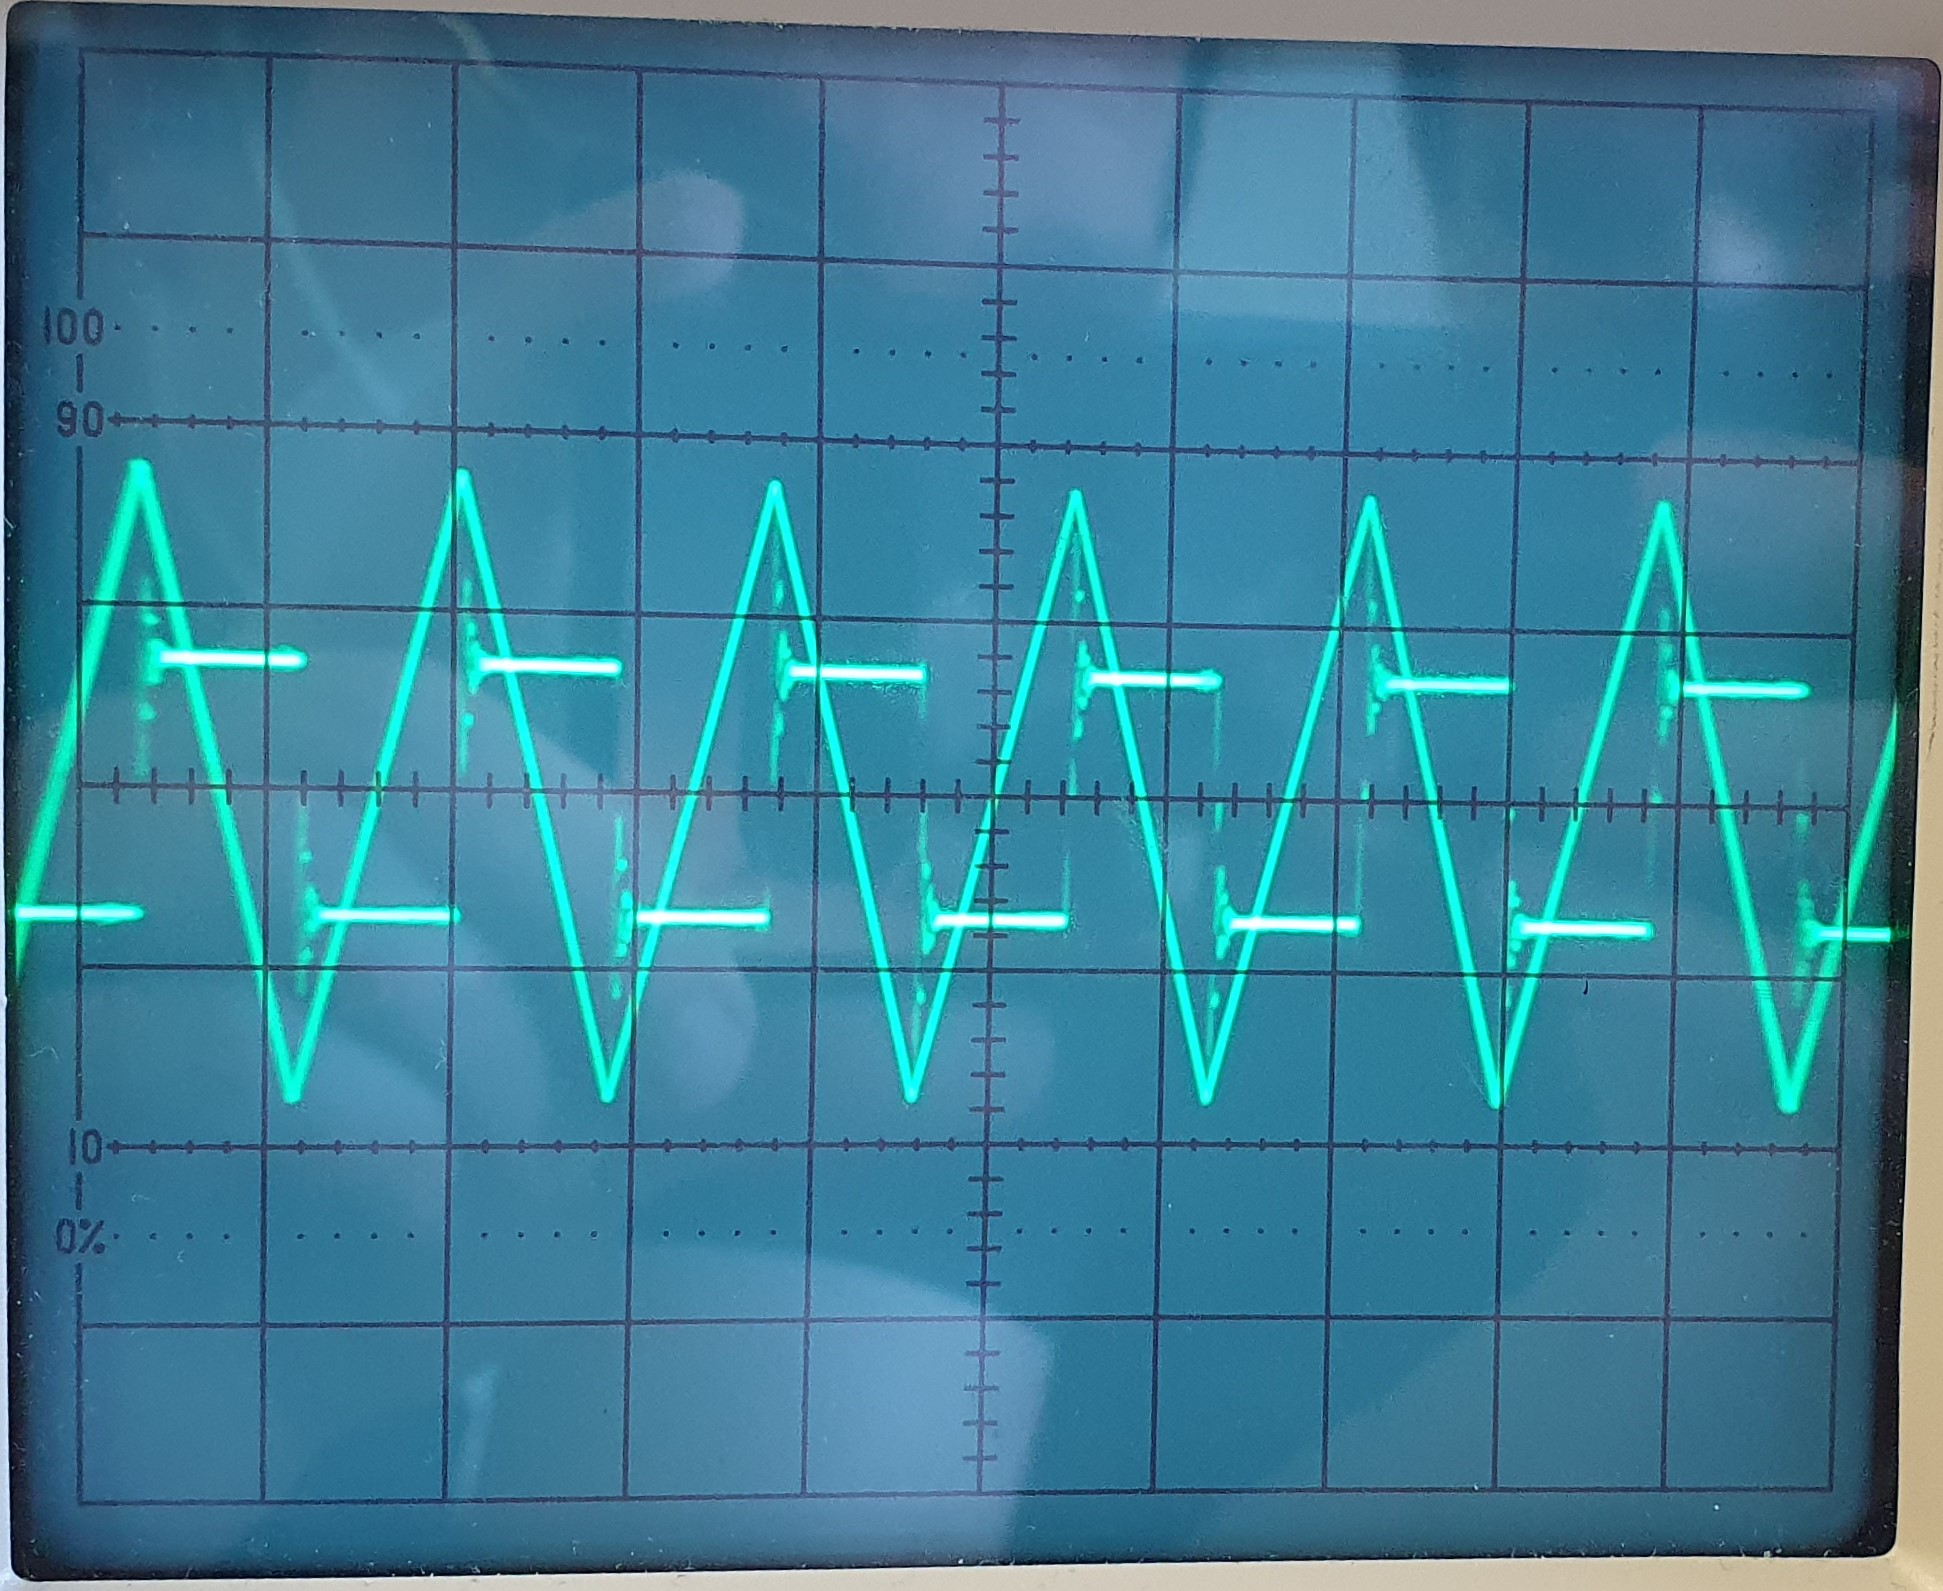
\includegraphics[scale=0.2]{64/(5) Differentierer, franzig_c.jpg}
    \caption{Eingangsspannung (Dreieck) und Ausgangsspannung (Rechteck) der einfachen Differenzierschaltung.}
\end{figure}\newpage
Bei genauerem Betrachten der Rechteckspannung fallen Störsignale auf. Die Ursache hierfür ist wahrscheinlich, wie in der Versuchsanleitung beschrieben, der komplexe Eingangswiderstand:
\begin{align}
    R_\text{e} = \frac{1}{\omega C_1}
\end{align}
Dieser sinkt nämlich mit steigender Frequenz, wodurch hochfrequente Störsignale leichter verstärkt werden.

Um Störungen zu vermeiden wird die Schaltung durch hinzufügen eines Widerstands und eines Kondensators folgendermaßen erweitert:
\begin{figure}[h]
    \centering\begin{circuitikz}[european resistors]
        \draw(0,0) node[op amp, yscale=-1] (opamp){};
        \draw (opamp.+) to [C=$C_1$]++(-1.25,0)to [R=$R_1$] ++(-1.25,0) to [short,-o]+(-0.5,0)to[open,v>=$U_\text{e}$] ++(0,-3) to [short,o-] ++(2,0) to node[ground](gnd){} ++(0,0);
        \draw (opamp.-) to [short] ++(-1,0) to [short] ++(0,-1) to node[short](r2){} ++(0,0) to [short,-*] (gnd);
        \draw (gnd) to [short,-o]++(5.35,0) to node[short,-o](end){}++(0,0);
        \draw (opamp.out) to node[short,*-*](r1){} ++(1,0) to [short,-o] ++(1,0) to [open,v>=$U_\text{a}$] (end);
        %\draw (r1) to [short,*-,i>^=$I_2$]++(0,-1.5) to [R=$R_2$,v>=$U_2$] (r2);
        %\draw (r2)++(0,1) to [open] ++(-1,0) to node[short](o1){} ++(0,0)to[open,v>=$U_1$]++(0,-3);
        %\draw (o1) to [open,v^<=$U_3$]++(0,1);
        \draw (opamp.out) to [short,*-*]  ++(0,2) to node[short](R2){}++(0,0) to [R=$R_2$]++(-2.35,0) to [short,*-*] (opamp.+);
        \draw (R2) to [short,*-]++(0,1.5) to [C=$C_2$]++(-2.35,0) to [short,-*] ++(0,-1.5);
    \end{circuitikz}
    \caption{Schaltplan der erweiterten Differenzierschaltung (Bandpass)}
\end{figure}\\
Bei erneutem Anlegen einer Dreiecksspannung, ergibt sich folgendes Bild auf dem Oszilloskop:
\begin{figure}[h]
    \centering
    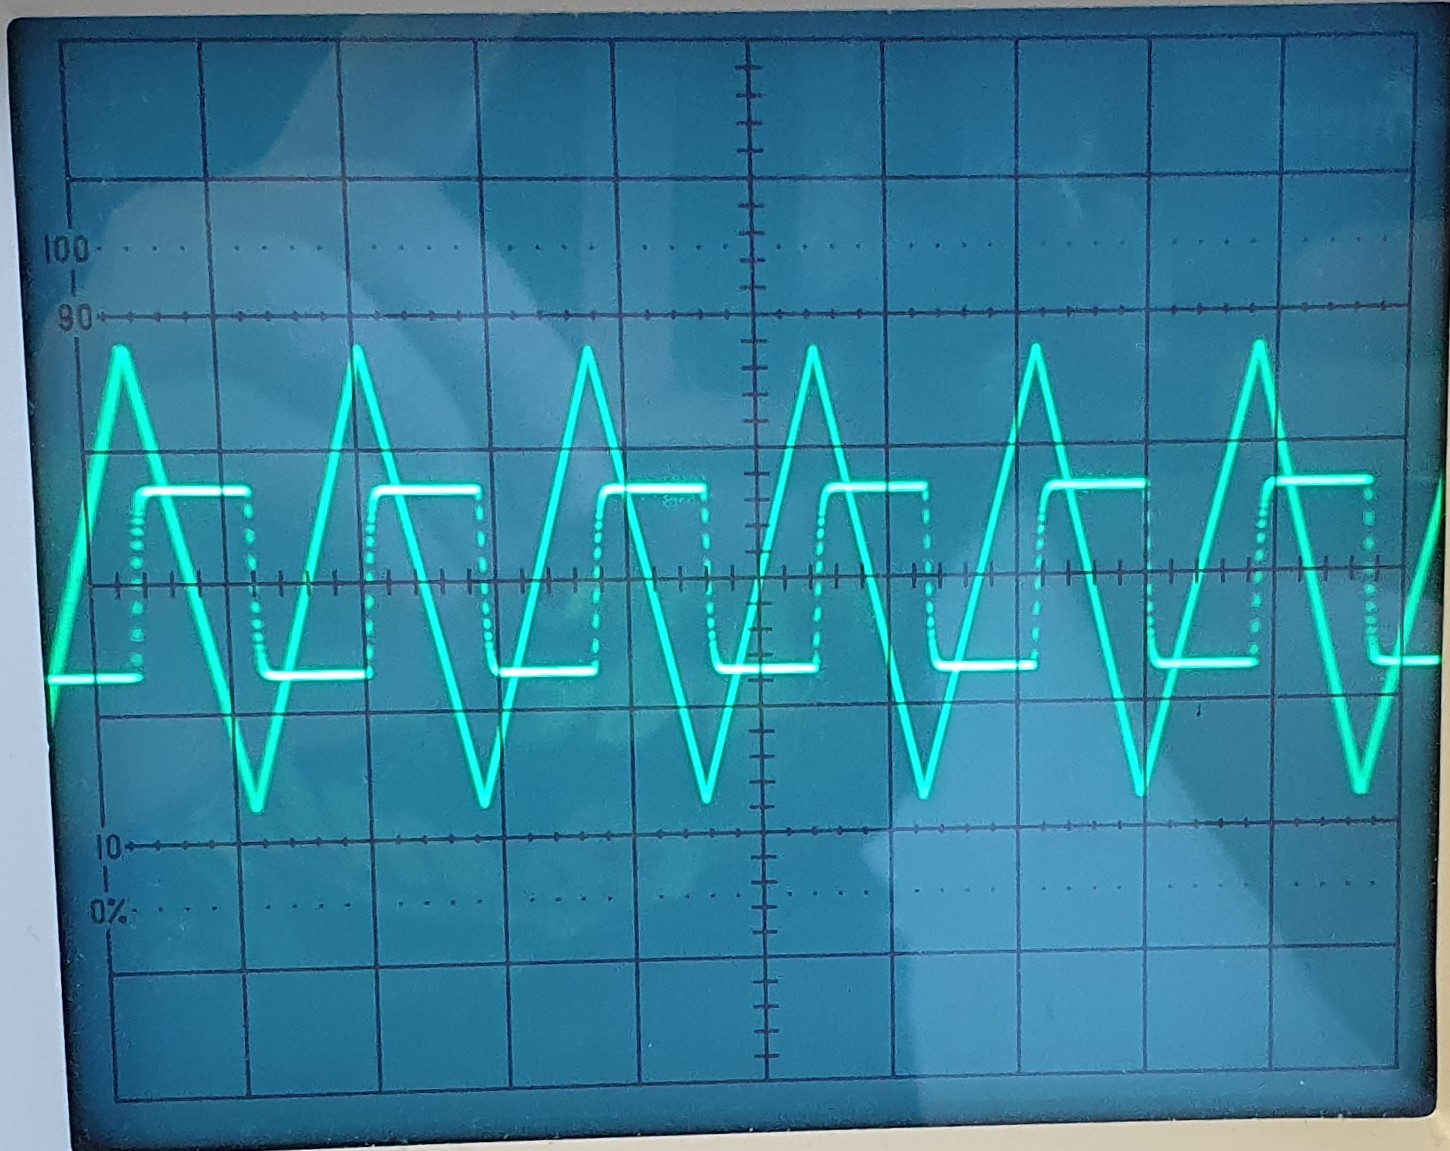
\includegraphics[scale=0.2]{64/(6) Differerntierer, normal (2)_c.jpg}
    \caption{Eingangsspannung (Dreieck) und Ausgangsspannung (Rechteck) der erweiterten Differenzierschaltung}
\end{figure}
\newpage
Durch einbauen von \(C_2\) und \(R_1\) wird die Verstärkung der hohen Frequenzen begrenzt, wodurch die Signalqualität wesentlich verbessert wird.

In unserem Fall verschwinden nicht nur die großen Störsignale zu Beginn eines Abschnitts der Rechteckspannung, sondern auch die allgemeine Liniendicke verringert sich.

Durch die Erweiterungen arbeitet die Schalung jedoch nur noch für bestimmte Frequenzen \(\omega \ll \omega_0\) als Differenzierer. Genaueres dazu wurde in Frage 5 der Fragen zur Vorbereitung besprochen.

Betrachtet man den Frequenzgang im Hinblick auf die Überlegungen aus Frage 5 der Fragen zur Vorbereitung, so ist, wie erwartet, in den Messdaten die Charakteristik eines Bandpasses zu erkennen.

Mit den Daten aus der vorherigen Aufgabe ergibt sich folgender Plot:
\begin{figure}[h]
    \centering\scalebox{1}{% GNUPLOT: LaTeX picture with Postscript
\begingroup
  % Encoding inside the plot.  In the header of your document, this encoding
  % should to defined, e.g., by using
  % \usepackage[cp1252,<other encodings>]{inputenc}
  \inputencoding{cp1252}%
  \makeatletter
  \providecommand\color[2][]{%
    \GenericError{(gnuplot) \space\space\space\@spaces}{%
      Package color not loaded in conjunction with
      terminal option `colourtext'%
    }{See the gnuplot documentation for explanation.%
    }{Either use 'blacktext' in gnuplot or load the package
      color.sty in LaTeX.}%
    \renewcommand\color[2][]{}%
  }%
  \providecommand\includegraphics[2][]{%
    \GenericError{(gnuplot) \space\space\space\@spaces}{%
      Package graphicx or graphics not loaded%
    }{See the gnuplot documentation for explanation.%
    }{The gnuplot epslatex terminal needs graphicx.sty or graphics.sty.}%
    \renewcommand\includegraphics[2][]{}%
  }%
  \providecommand\rotatebox[2]{#2}%
  \@ifundefined{ifGPcolor}{%
    \newif\ifGPcolor
    \GPcolorfalse
  }{}%
  \@ifundefined{ifGPblacktext}{%
    \newif\ifGPblacktext
    \GPblacktexttrue
  }{}%
  % define a \g@addto@macro without @ in the name:
  \let\gplgaddtomacro\g@addto@macro
  % define empty templates for all commands taking text:
  \gdef\gplbacktext{}%
  \gdef\gplfronttext{}%
  \makeatother
  \ifGPblacktext
    % no textcolor at all
    \def\colorrgb#1{}%
    \def\colorgray#1{}%
  \else
    % gray or color?
    \ifGPcolor
      \def\colorrgb#1{\color[rgb]{#1}}%
      \def\colorgray#1{\color[gray]{#1}}%
      \expandafter\def\csname LTw\endcsname{\color{white}}%
      \expandafter\def\csname LTb\endcsname{\color{black}}%
      \expandafter\def\csname LTa\endcsname{\color{black}}%
      \expandafter\def\csname LT0\endcsname{\color[rgb]{1,0,0}}%
      \expandafter\def\csname LT1\endcsname{\color[rgb]{0,1,0}}%
      \expandafter\def\csname LT2\endcsname{\color[rgb]{0,0,1}}%
      \expandafter\def\csname LT3\endcsname{\color[rgb]{1,0,1}}%
      \expandafter\def\csname LT4\endcsname{\color[rgb]{0,1,1}}%
      \expandafter\def\csname LT5\endcsname{\color[rgb]{1,1,0}}%
      \expandafter\def\csname LT6\endcsname{\color[rgb]{0,0,0}}%
      \expandafter\def\csname LT7\endcsname{\color[rgb]{1,0.3,0}}%
      \expandafter\def\csname LT8\endcsname{\color[rgb]{0.5,0.5,0.5}}%
    \else
      % gray
      \def\colorrgb#1{\color{black}}%
      \def\colorgray#1{\color[gray]{#1}}%
      \expandafter\def\csname LTw\endcsname{\color{white}}%
      \expandafter\def\csname LTb\endcsname{\color{black}}%
      \expandafter\def\csname LTa\endcsname{\color{black}}%
      \expandafter\def\csname LT0\endcsname{\color{black}}%
      \expandafter\def\csname LT1\endcsname{\color{black}}%
      \expandafter\def\csname LT2\endcsname{\color{black}}%
      \expandafter\def\csname LT3\endcsname{\color{black}}%
      \expandafter\def\csname LT4\endcsname{\color{black}}%
      \expandafter\def\csname LT5\endcsname{\color{black}}%
      \expandafter\def\csname LT6\endcsname{\color{black}}%
      \expandafter\def\csname LT7\endcsname{\color{black}}%
      \expandafter\def\csname LT8\endcsname{\color{black}}%
    \fi
  \fi
    \setlength{\unitlength}{0.0500bp}%
    \ifx\gptboxheight\undefined%
      \newlength{\gptboxheight}%
      \newlength{\gptboxwidth}%
      \newsavebox{\gptboxtext}%
    \fi%
    \setlength{\fboxrule}{0.5pt}%
    \setlength{\fboxsep}{1pt}%
\begin{picture}(7200.00,5040.00)%
    \gplgaddtomacro\gplbacktext{%
      \csname LTb\endcsname%%
      \put(946,704){\makebox(0,0)[r]{\strut{}$0.01$}}%
      \put(946,1439){\makebox(0,0)[r]{\strut{}$0.1$}}%
      \put(946,2173){\makebox(0,0)[r]{\strut{}$1$}}%
      \put(946,2908){\makebox(0,0)[r]{\strut{}$10$}}%
      \put(946,3642){\makebox(0,0)[r]{\strut{}$100$}}%
      \put(946,4377){\makebox(0,0)[r]{\strut{}$1000$}}%
      \put(1078,484){\makebox(0,0){\strut{}$1$}}%
      \put(1969,484){\makebox(0,0){\strut{}$10$}}%
      \put(2860,484){\makebox(0,0){\strut{}$100$}}%
      \put(3751,484){\makebox(0,0){\strut{}$1000$}}%
      \put(4642,484){\makebox(0,0){\strut{}$10000$}}%
      \put(5534,484){\makebox(0,0){\strut{}$100000$}}%
      \put(6425,484){\makebox(0,0){\strut{}$1\times10^{6}$}}%
    }%
    \gplgaddtomacro\gplfronttext{%
      \csname LTb\endcsname%%
      \put(209,2761){\rotatebox{-270}{\makebox(0,0){\strut{}$\nu$}}}%
      \csname LTb\endcsname%%
      \put(6748,2761){\rotatebox{-270}{\makebox(0,0){\strut{}}}}%
      \csname LTb\endcsname%%
      \put(3885,154){\makebox(0,0){\strut{}$\omega\,\left(\frac{1}{\text{s}}\right)$}}%
      \csname LTb\endcsname%%
      \put(3885,4819){\makebox(0,0){\strut{}}}%
      \csname LTb\endcsname%%
      \put(132,-110){\makebox(0,0)[l]{\strut{}}}%
      \csname LTb\endcsname%%
      \put(5706,4646){\makebox(0,0)[r]{\strut{}Messwerte - (6.3)}}%
      \csname LTb\endcsname%%
      \put(5706,4426){\makebox(0,0)[r]{\strut{}Erwartete Werte - (6.3)}}%
      \csname LTb\endcsname%%
      \put(5706,4206){\makebox(0,0)[r]{\strut{}Messwerte - (6.4)}}%
      \csname LTb\endcsname%%
      \put(3885,135175){\makebox(0,0){\strut{}}}%
    }%
    \gplbacktext
    \put(0,0){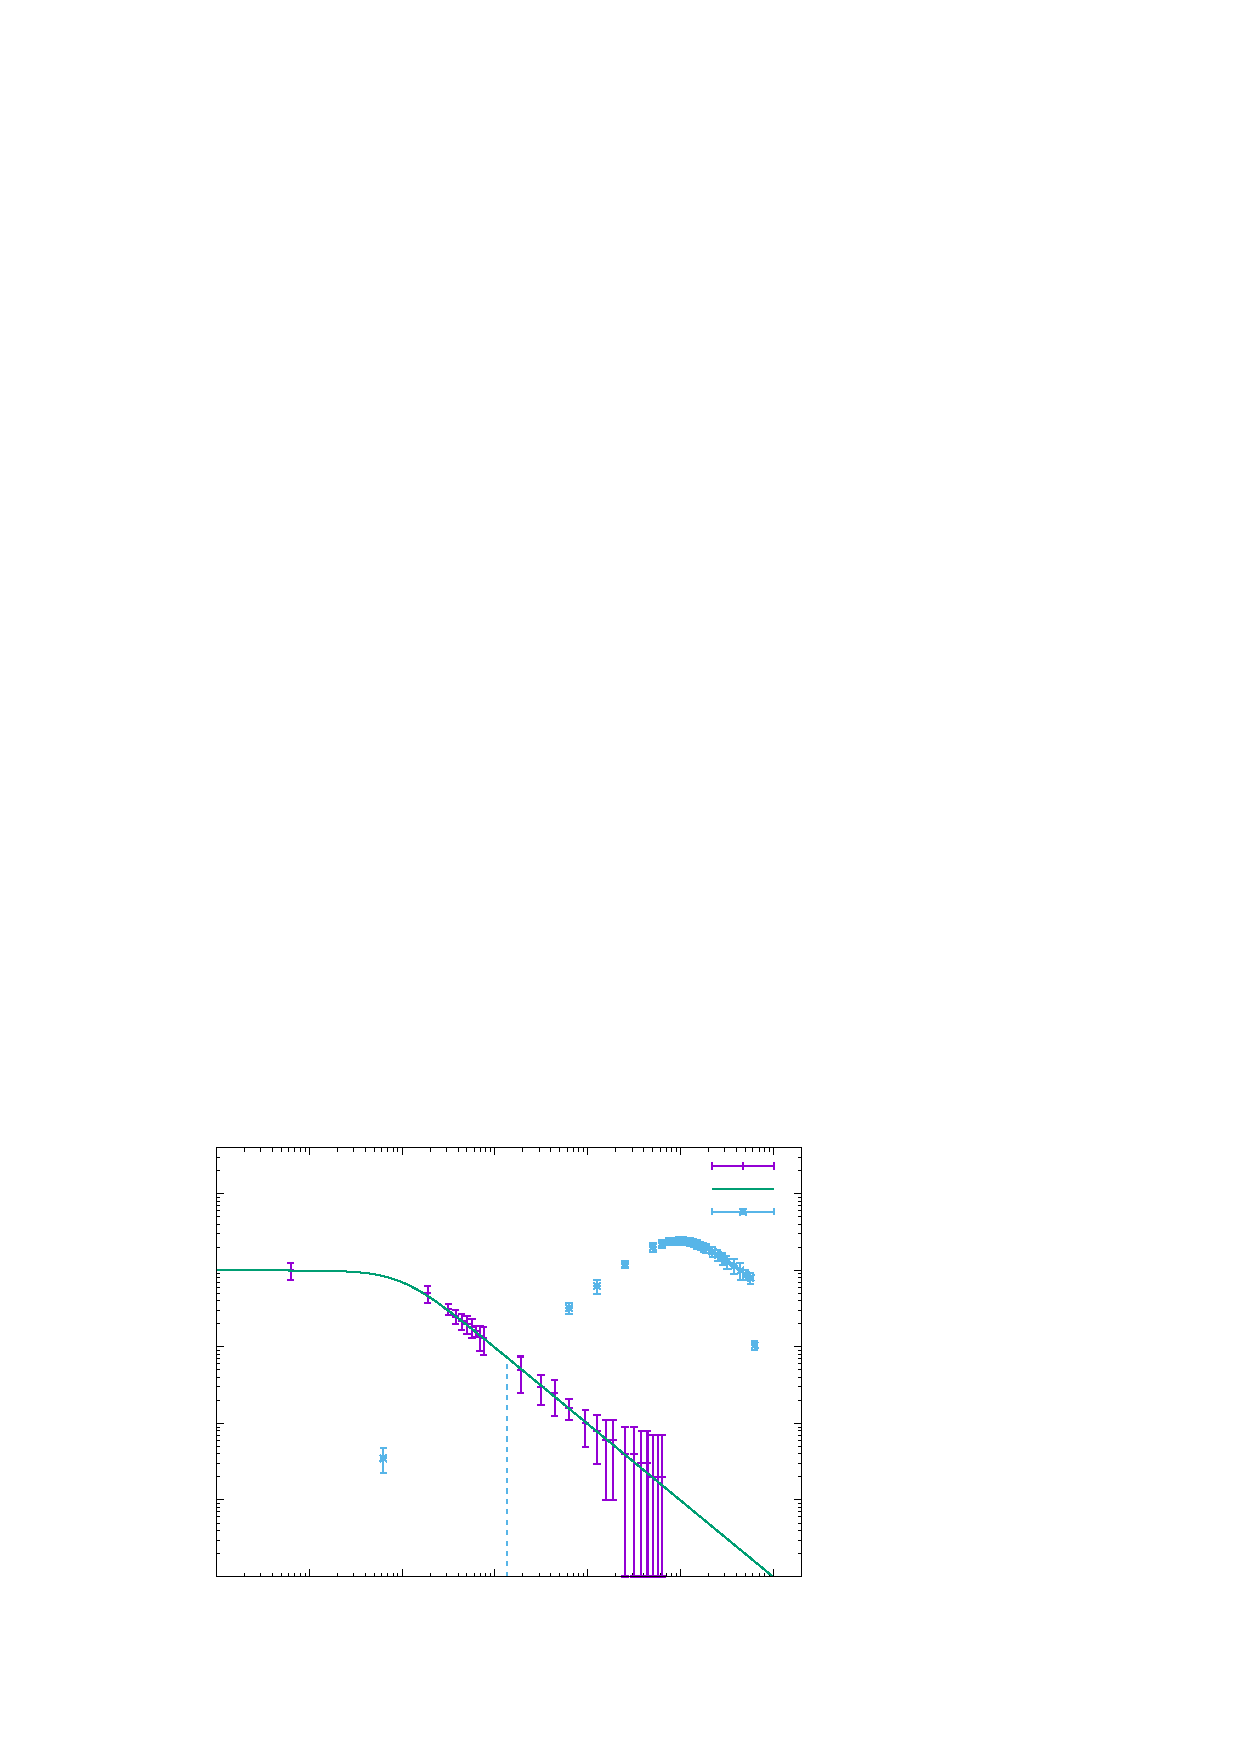
\includegraphics[width={360.00bp},height={252.00bp}]{Differenzierer_final}}%
    \gplfronttext
  \end{picture}%
\endgroup
}
    \caption{Frequenzgang des Bandpasses (blau) und Umkehrintegrators (lila)}
\end{figure}\\
Die Kurven schneiden sich bei einer Frequenz von \(\omega \approx 1330\,\frac{1}{\text{s}}\), da die Schaltung des Bandpasses links von seinem Hochpunkt als Integrierer arbeitet und ermöglicht somit einen Schnittpunkt.
Zudem sind die Grenzfrequenzen aufgrund der unterschiedlichen verwendeten Bauteile verschoben.
\newpage
\textbf{Verbesserung}\\
% Table generated by Excel2LaTeX from sheet 'Tabelle1'
\begin{table}[htbp]
    \centering
      \begin{tabular}{c|c|c|c}
        $\omega$ in $\frac{1}{\text{s}}$ & $s_\omega$ in $\frac{1}{\text{s}}$ & $\nu$ & $s_\nu$\\
        \hline
      62,8318531 & 0,02513274 & 0,007 & 0,00250881 \\
      6283,18531 & 2,51327412 & 0,64 & 0,10182775 \\
      12566,3706 & 5,02654825 & 1,25 & 0,25279874 \\
      25132,7412 & 10,0530965 & 2,4 & 0,26016824 \\
      50265,4825 & 20,106193 & 4,0 & 0,5142079 \\
      62831,8531 & 25,1327412 & 4,5 & 0,51791636 \\
      75398,2237 & 30,1592895 & 4,8 & 0,52033648 \\
      81681,409 & 32,6725636 & 4,8 & 0,52033648 \\
      87964,5943 & 35,1858377 & 4,8 & 0,52033648 \\
      94247,7796 & 37,6991118 & 4,9 & 0,52117525 \\
      100530,965 & 40,212386 & 4,9 & 0,52117525 \\
      106814,15 & 42,7256601 & 4,9 & 0,52117525 \\
      113097,336 & 45,2389342 & 4,8 & 0,52033648 \\
      119380,521 & 47,7522083 & 4,8 & 0,52033648 \\
      125663,706 & 50,2654825 & 4,7 & 0,51951369 \\
      138230,077 & 55,2920307 & 4,6 & 0,51870696 \\
      150796,447 & 60,3185789 & 4,4 & 0,51714196 \\
      163362,818 & 65,3451272 & 4,2 & 0,51564209 \\
      175929,189 & 70,3716754 & 4,0 & 0,5142079 \\
      188495,559 & 75,3982237 & 3,9 & 0,51351561 \\
      219911,486 & 87,9645943 & 3,5 & 0,51091337 \\
      251327,412 & 100,530965 & 3,2 & 0,50913873 \\
      282743,339 & 113,097336 & 2,9 & 0,50751762 \\
      314159,265 & 125,663706 & 2,6 & 0,5060515 \\
      376991,118 & 150,796447 & 2,3 & 0,50474174 \\
      439822,972 & 175,929189 & 2 & 0,50358956 \\
      502654,825 & 201,06193 & 1,75 & 0,25545669 \\
      565486,678 & 226,194671 & 1,6 & 0,25456937 \\
      628318,531 & 251,327412 & 0,21 & 0,0257821 \\
      \end{tabular}%
      \caption{Wertetabelle Differenzierschaltung}
  \end{table}\newpage
  Angepasster Plot:
\begin{figure}[h]
    \centering\scalebox{1}{% GNUPLOT: LaTeX picture with Postscript
\begingroup
  % Encoding inside the plot.  In the header of your document, this encoding
  % should to defined, e.g., by using
  % \usepackage[cp1252,<other encodings>]{inputenc}
  \inputencoding{cp1252}%
  \makeatletter
  \providecommand\color[2][]{%
    \GenericError{(gnuplot) \space\space\space\@spaces}{%
      Package color not loaded in conjunction with
      terminal option `colourtext'%
    }{See the gnuplot documentation for explanation.%
    }{Either use 'blacktext' in gnuplot or load the package
      color.sty in LaTeX.}%
    \renewcommand\color[2][]{}%
  }%
  \providecommand\includegraphics[2][]{%
    \GenericError{(gnuplot) \space\space\space\@spaces}{%
      Package graphicx or graphics not loaded%
    }{See the gnuplot documentation for explanation.%
    }{The gnuplot epslatex terminal needs graphicx.sty or graphics.sty.}%
    \renewcommand\includegraphics[2][]{}%
  }%
  \providecommand\rotatebox[2]{#2}%
  \@ifundefined{ifGPcolor}{%
    \newif\ifGPcolor
    \GPcolorfalse
  }{}%
  \@ifundefined{ifGPblacktext}{%
    \newif\ifGPblacktext
    \GPblacktexttrue
  }{}%
  % define a \g@addto@macro without @ in the name:
  \let\gplgaddtomacro\g@addto@macro
  % define empty templates for all commands taking text:
  \gdef\gplbacktext{}%
  \gdef\gplfronttext{}%
  \makeatother
  \ifGPblacktext
    % no textcolor at all
    \def\colorrgb#1{}%
    \def\colorgray#1{}%
  \else
    % gray or color?
    \ifGPcolor
      \def\colorrgb#1{\color[rgb]{#1}}%
      \def\colorgray#1{\color[gray]{#1}}%
      \expandafter\def\csname LTw\endcsname{\color{white}}%
      \expandafter\def\csname LTb\endcsname{\color{black}}%
      \expandafter\def\csname LTa\endcsname{\color{black}}%
      \expandafter\def\csname LT0\endcsname{\color[rgb]{1,0,0}}%
      \expandafter\def\csname LT1\endcsname{\color[rgb]{0,1,0}}%
      \expandafter\def\csname LT2\endcsname{\color[rgb]{0,0,1}}%
      \expandafter\def\csname LT3\endcsname{\color[rgb]{1,0,1}}%
      \expandafter\def\csname LT4\endcsname{\color[rgb]{0,1,1}}%
      \expandafter\def\csname LT5\endcsname{\color[rgb]{1,1,0}}%
      \expandafter\def\csname LT6\endcsname{\color[rgb]{0,0,0}}%
      \expandafter\def\csname LT7\endcsname{\color[rgb]{1,0.3,0}}%
      \expandafter\def\csname LT8\endcsname{\color[rgb]{0.5,0.5,0.5}}%
    \else
      % gray
      \def\colorrgb#1{\color{black}}%
      \def\colorgray#1{\color[gray]{#1}}%
      \expandafter\def\csname LTw\endcsname{\color{white}}%
      \expandafter\def\csname LTb\endcsname{\color{black}}%
      \expandafter\def\csname LTa\endcsname{\color{black}}%
      \expandafter\def\csname LT0\endcsname{\color{black}}%
      \expandafter\def\csname LT1\endcsname{\color{black}}%
      \expandafter\def\csname LT2\endcsname{\color{black}}%
      \expandafter\def\csname LT3\endcsname{\color{black}}%
      \expandafter\def\csname LT4\endcsname{\color{black}}%
      \expandafter\def\csname LT5\endcsname{\color{black}}%
      \expandafter\def\csname LT6\endcsname{\color{black}}%
      \expandafter\def\csname LT7\endcsname{\color{black}}%
      \expandafter\def\csname LT8\endcsname{\color{black}}%
    \fi
  \fi
    \setlength{\unitlength}{0.0500bp}%
    \ifx\gptboxheight\undefined%
      \newlength{\gptboxheight}%
      \newlength{\gptboxwidth}%
      \newsavebox{\gptboxtext}%
    \fi%
    \setlength{\fboxrule}{0.5pt}%
    \setlength{\fboxsep}{1pt}%
\begin{picture}(7200.00,5040.00)%
    \gplgaddtomacro\gplbacktext{%
      \csname LTb\endcsname%%
      \put(946,704){\makebox(0,0)[r]{\strut{}$0.01$}}%
      \put(946,1439){\makebox(0,0)[r]{\strut{}$0.1$}}%
      \put(946,2173){\makebox(0,0)[r]{\strut{}$1$}}%
      \put(946,2908){\makebox(0,0)[r]{\strut{}$10$}}%
      \put(946,3642){\makebox(0,0)[r]{\strut{}$100$}}%
      \put(946,4377){\makebox(0,0)[r]{\strut{}$1000$}}%
      \put(1078,484){\makebox(0,0){\strut{}$1$}}%
      \put(1969,484){\makebox(0,0){\strut{}$10$}}%
      \put(2860,484){\makebox(0,0){\strut{}$100$}}%
      \put(3751,484){\makebox(0,0){\strut{}$1000$}}%
      \put(4642,484){\makebox(0,0){\strut{}$10000$}}%
      \put(5534,484){\makebox(0,0){\strut{}$100000$}}%
      \put(6425,484){\makebox(0,0){\strut{}$1\times10^{6}$}}%
    }%
    \gplgaddtomacro\gplfronttext{%
      \csname LTb\endcsname%%
      \put(209,2761){\rotatebox{-270}{\makebox(0,0){\strut{}$\nu$}}}%
      \csname LTb\endcsname%%
      \put(6748,2761){\rotatebox{-270}{\makebox(0,0){\strut{}}}}%
      \csname LTb\endcsname%%
      \put(3885,154){\makebox(0,0){\strut{}$\omega\,\left(\frac{1}{\text{s}}\right)$}}%
      \csname LTb\endcsname%%
      \put(3885,4819){\makebox(0,0){\strut{}}}%
      \csname LTb\endcsname%%
      \put(132,-110){\makebox(0,0)[l]{\strut{}}}%
      \csname LTb\endcsname%%
      \put(5706,4646){\makebox(0,0)[r]{\strut{}Erwartete Werte}}%
      \csname LTb\endcsname%%
      \put(5706,4426){\makebox(0,0)[r]{\strut{}Messwerte}}%
      \csname LTb\endcsname%%
      \put(5706,4206){\makebox(0,0)[r]{\strut{}Erwartete Werte - (6.4)}}%
      \csname LTb\endcsname%%
      \put(3885,45225){\makebox(0,0){\strut{}}}%
    }%
    \gplbacktext
    \put(0,0){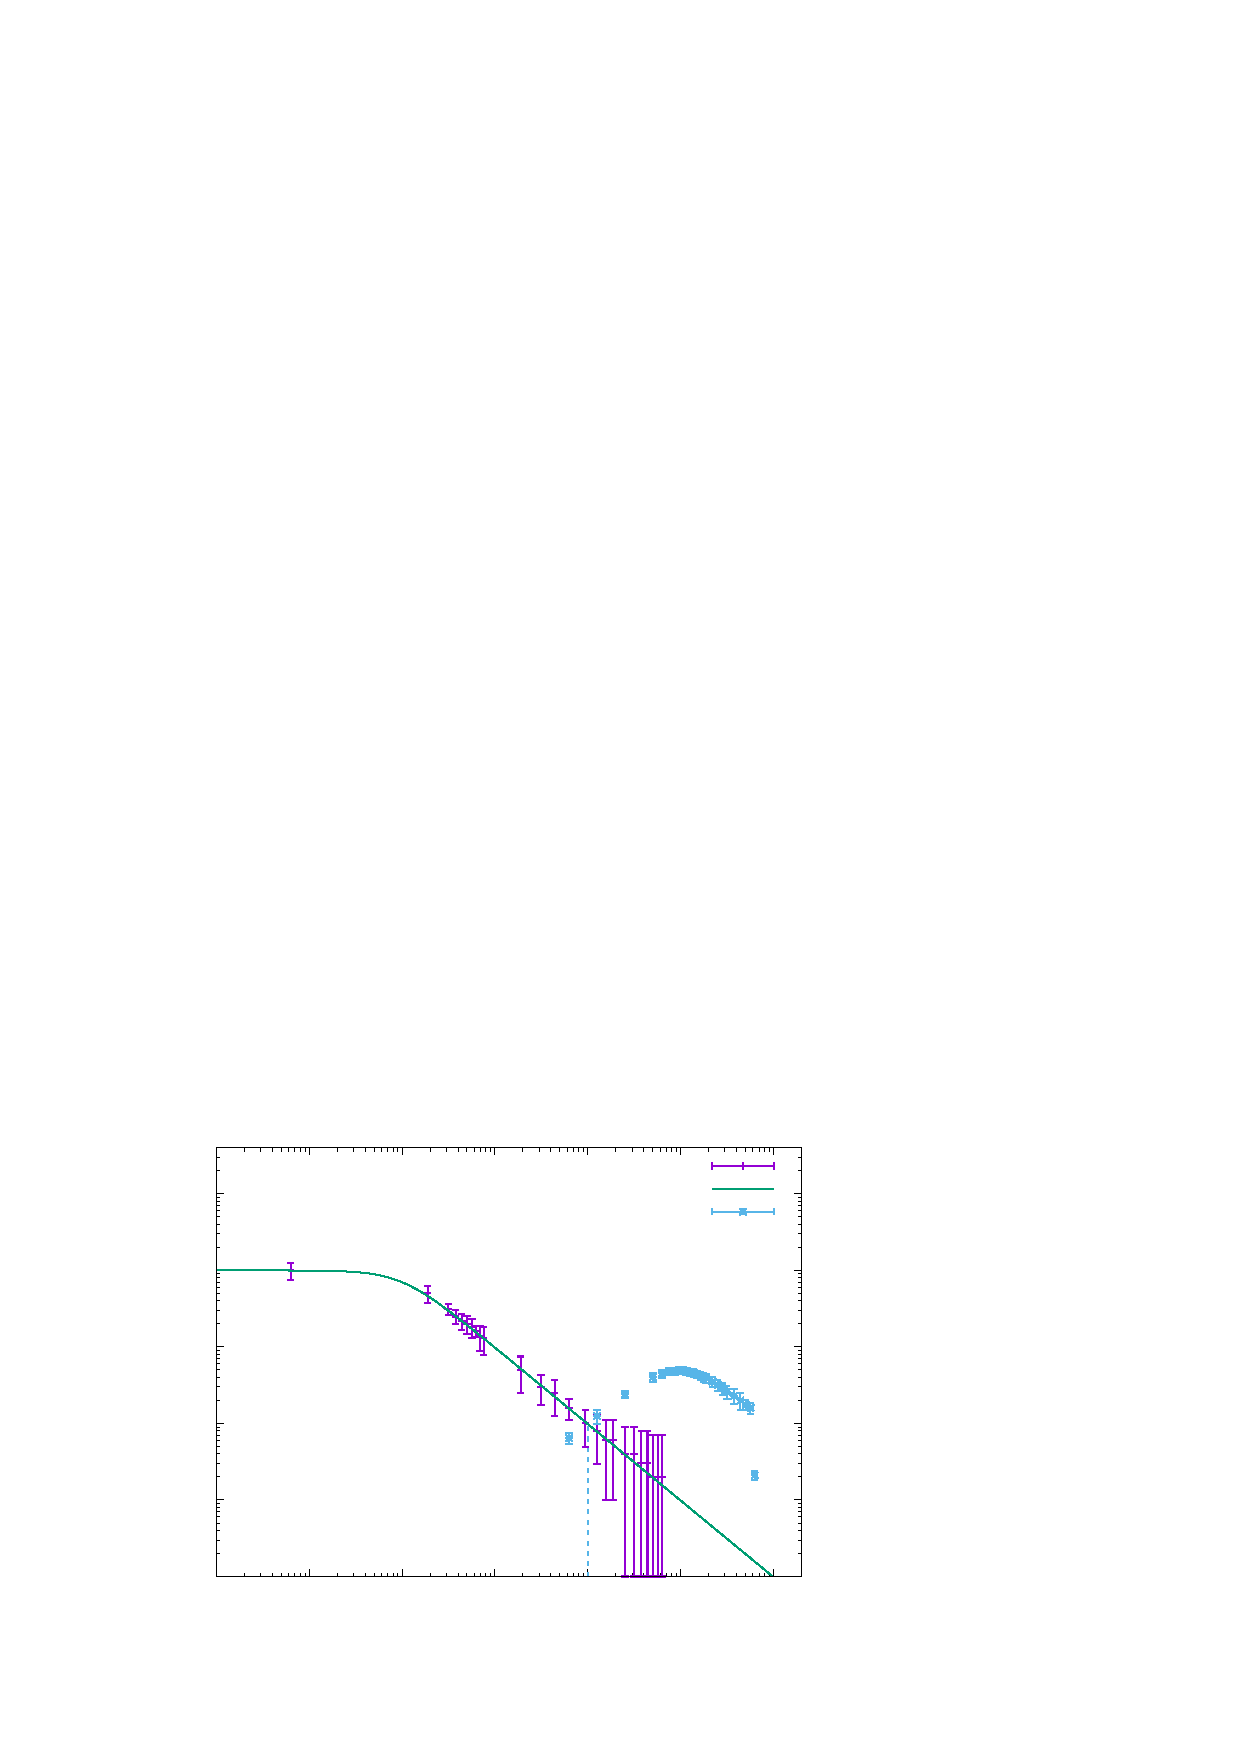
\includegraphics[width={360.00bp},height={252.00bp}]{diff-verb}}%
    \gplfronttext
  \end{picture}%
\endgroup
}
    \caption{Frequenzgang des Bandpasses (blau) und Umkehrintegrators (lila)}
\end{figure}